%!TEX root = ../template.tex
%%%%%%%%%%%%%%%%%%%%%%%%%%%%%%%%%%%%%%%%%%%%%%%%%%%%%%%%%%%%%%%%%%%
%% 5 - Methodology.tex
%% NOVA thesis document file
%%
%% Chapter with Methodology
%%%%%%%%%%%%%%%%%%%%%%%%%%%%%%%%%%%%%%%%%%%%%%%%%%%%%%%%%%%%%%%%%%%
% chktex-file 24
\typeout{NT FILE 5 - Methodology}%

\chapter{Methodology}
\label{cha:methodology}

This chapter describes the methodology used to evaluate the testbed described in Chapter~\ref{cha:proposed-architecture}. Section~\ref{sec:experimental-testbed} describes the three test locations, their distances from the radio and the obstructions on each path. Section~\ref{sec:experimental-methodology} describes the traffic conditions used at each location, and the \gls{TDD} structures the 5G \gls{RAN} was configured with. Section~\ref{sec:experiments} describes the three test rounds, and the configuration changes made between them. The results of these tests will follow in Chapter~\ref{cha:results}.

\section{Experimental Testbed}
\label{sec:experimental-testbed}
The network's performance was evaluated at three fixed \gls{UE} positions in the same room as the \gls{RAN}, chosen to combine increasing distance from the radio with different obstruction conditions at each point. Figure~\ref{fig:lab-floor-plan} shows the top plan view of the room, and Figure~\ref{fig:test-location-heights} shows the elevation, giving the height of the radio and of the \gls{UE} at each location above the floor.

Material and thickness are recorded for each obstruction as they, and not distance alone, also account for the difference between the three locations: signal attenuation through a wall depends strongly on its material and thickness, particularly at the 3.4\,GHz centre frequency used by the 5G \gls{RAN}, so the three locations should be read as distance-plus-obstruction conditions rather than a simple distance variation. Figure~\ref{fig:thickness-collage} shows the tape-measure readings taken for both obstructions.

\begin{figure}
    \centering
    
\includegraphics[width=1\textwidth]{Lab_Floor_Plan.pdf}
    \caption{Plan view of the room, showing the radio position and the three \gls{UE} test locations, drawn to scale.}
    \label{fig:lab-floor-plan}
\end{figure}

\begin{figure}
    \centering
    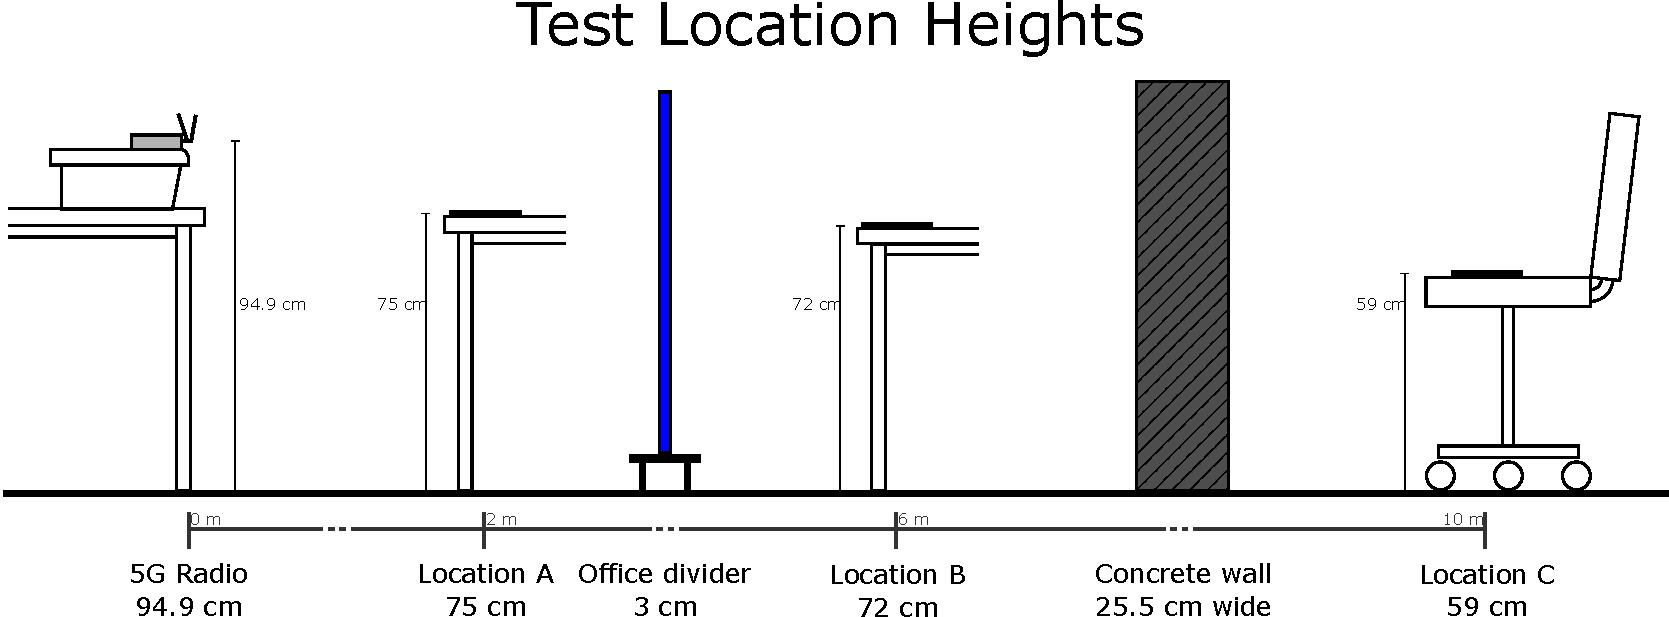
\includegraphics[width=0.9\textwidth]{Heights.pdf}
    \caption[Elevation view of the radio and UE heights]{Elevation view showing the mounting height of the radio and the \gls{UE} height at each test location, along with the obstruction on the path to locations B and C.}
    \label{fig:test-location-heights}
\end{figure}

\begin{figure}
    \centering
    
\includegraphics[width=0.95\textwidth]{thickness_collage.jpg}
    \caption[Measured thickness of the two obstructions]{Tape measured thickness readings for the two obstructions on the direct path: the concrete wall at Location C (25.3\,cm) and the office partition at Location B (3\,cm).}
    \label{fig:thickness-collage}
\end{figure}

Besides obstructions, the objects present in the room may account for signal attenuation as well. In Figure~\ref{fig:lab-floor-plan}, the objects shown in dark grey are metal furniture and equipment present in the room. None of these lie directly on the signal path between the \gls{RAN} and any of the three test locations, but their metal construction means they may still have contributed to reflections and multipath propagation, and should be kept in mind when interpreting the results. Other objects present in the room, such as the tables and doors shown on the diagram, present minimal attenuation and are not expected to have a significant effect on the results.
A summary of all measurements and signal obstruction conditions for each of the three test locations is presented in Table~\ref{tab:test-locations}.
% These measurements are also intended to support a comparison between the obstructions' theoretical attenuation and the attenuation actually observed in the collected data.

\begin{table}[htbp]
    \centering
    \begin{tabular}{|c|c|c|c|c|c|}
        \hline
        \textbf{Location} & \textbf{Distance} & \textbf{Height} & \textbf{Obstruction} & \textbf{Material}& \textbf{Thickness} \\
        \hline
        A & 2\,m  & 75\,cm & Clear line of sight & --- & --- \\
        \hline
        B & 6\,m  & 72\,cm & Office partition & Plastic and Felt & 3\,cm \\
        \hline
        C & 10\,m & 59\,cm & Concrete wall & Concrete & 25.3\,cm \\
        \hline
    \end{tabular}
    \caption[The three test locations]{The three test locations: distance from the radio, \gls{UE} height above the floor, the obstruction material and thickness on the direct path at each point. All distances, thicknesses and heights were measured directly with a tape measure.}
    \label{tab:test-locations}
\end{table}

\newpage

\section{Experimental Methodology}
\label{sec:experimental-methodology}
At each location, tests were run for each generation of network, for both TCP and UDP, and for both uplink and downlink, giving four traffic conditions per location, per generation. For the 4G network, each of these conditions was tested once ($n=1$); for the 5G network, each was repeated three times ($n=3$). This difference was not a deliberate methodological choice about sample size per generation: the 4G network was only tested during the first round of testing, in which every combination, both in 4G and 5G, was only tested once. Subsequent rounds of testing focused exclusively on the 5G network, following configuration corrections described later in this chapter, and used three repetitions per condition from that point onward; the 4G network was deliberately left untouched throughout, so its results were never repeated.

Traffic was generated with \texttt{iperf3}, with the server running on the core machine and the client running on the \gls{UE} through the CellularLab app~\cite{cellularlab}, which provides an \texttt{iperf3} client for Android devices. Each test consisted of a single 20-second \texttt{iperf3} run, over either TCP or UDP, in either the uplink or the downlink direction. To saturate the link, the client opened eight parallel streams. TCP tests used the default \texttt{iperf3} parameters, while UDP tests set a target rate of 100\,Mbps per stream (\texttt{-b 100M}), roughly 800\,Mbps in total. This is well above the capacity of either network, so the measured UDP throughput reflects what the link can carry at its maximum, rather than the rate that was offered. The results of each run were recorded both on the \gls{UE} and on the server.

Figure~\ref{fig:photo-locations} shows the three test locations as they were used for testing, with the \gls{UE} in place.

Initially, the 5G network was configured with a 3:1 \gls{TDD} structure. As specified by TS 38.213~\cite{3GPP38213} and described in Section~\ref{sec:ran_features}, the \gls{TDD} structure is defined by the TDD-UL-DL-ConfigurationCommon parameter, which is the \texttt{tdd\_ul\_dl\_cfg} block of the srsRAN \gls{gNB} configuration file, shown in Listing~\ref{lst:tdd-31-cfg}.
\newpage

\begin{figure}[htbp]
    \centering
    
\includegraphics[width=\textwidth]{locations_collage.jpg}
    \caption[The three test locations, with the UE in place]{The three test locations, with the \gls{UE} in place: Location A, 2\,m, clear line of sight;  Location B, 6\,m, behind the office partition; Location C, 10\,m, behind the concrete wall.}
    \label{fig:photo-locations}
\end{figure}

\begin{lstlisting}[language=yaml,backgroundcolor=\color{gray!20},frame=single,framerule=0.8pt,rulecolor=\color{black},basicstyle=\ttfamily\small,caption={\texttt{gnb.yaml} TDD configuration for the 3:1 pattern used in Round 1.},label={lst:tdd-31-cfg}]
tdd_ul_dl_cfg:
  dl_ul_tx_period: 5
  nof_dl_slots: 3
  nof_dl_symbols: 6
  nof_ul_slots: 1
  nof_ul_symbols: 2
\end{lstlisting}

This configuration dictates that for every 5-slot period, 3 slots are allocated for downlink and 1 slot is allocated for uplink, with the remaining flexible slot composed as follows: 6 symbols for downlink, 2 symbols for uplink and the remainder (6 symbols) are flexible. In total, given that a slot has 14 symbols, the total number of symbols per period is 70, with 48 symbols ($3\times14$ symbols + 6 symbols) allocated for downlink and 16 symbols ($1\times14$ symbols + 2 symbols) allocated for uplink. That gives 68.6\% of airtime for downlink and 22.9\% for uplink per period of transmission, with the remaining airtime being guard period.

Figure~\ref{fig:tdd-31-structure} shows the slot and symbol structure of the 5-slot period of the 3:1 \gls{TDD} pattern, which was used in Round 1.

\begin{figure}[htbp]
    \centering
    
\includegraphics[width=\textwidth]{TDD_3-1_Structure.pdf}
    \caption{Slot and symbol structure of the 3:1 TDD pattern used in Round 1.}
    \label{fig:tdd-31-structure}
\end{figure}

This structure was later found to impose a hard structural cap on uplink airtime, independent of signal quality, and was rebalanced to a symmetrical 2:2 structure from Round 2 onward, which meant that each transmission period was composed of two full downlink slots and two full uplink slots, along with a symmetrical flexible slot. Listing~\ref{lst:tdd-22-cfg} shows the corresponding \texttt{tdd\_ul\_dl\_cfg} block.

\begin{lstlisting}[language=yaml,backgroundcolor=\color{gray!20},frame=single,framerule=0.8pt,rulecolor=\color{black},basicstyle=\ttfamily\small,caption={\texttt{gnb.yaml} TDD configuration for the rebalanced 2:2 pattern used from Round 2 onward.},label={lst:tdd-22-cfg}]
tdd_ul_dl_cfg:
  dl_ul_tx_period: 5
  nof_dl_slots: 2
  nof_dl_symbols: 5
  nof_ul_slots: 2
  nof_ul_symbols: 5
\end{lstlisting}
With this configuration, out of the 70 total symbols per period, 33 symbols ($2\times14$ symbols + 5 symbols) are equally assigned to both downlink and uplink, giving 47.1\% of airtime for each direction, with the remaining airtime being guard period.

Figure~\ref{fig:tdd-22-structure} shows the resulting slot and symbol structure.

\begin{figure}[htbp]
    \centering
    
\includegraphics[width=\textwidth]{TDD_2-2_Structure.pdf}
    \caption{Slot and symbol structure of the rebalanced 5-slot period of the 2:2 TDD pattern used from Round 2 onward.}
    \label{fig:tdd-22-structure}
\end{figure}

All together, the rebalance is expected to roughly double the uplink airtime available to the scheduler ($22.9\% \rightarrow 47.1\% = \times2.06$) while reducing the downlink share to little more than two-thirds of what it was under the 3:1 pattern ($68.6\% \rightarrow 47.1\% = \times0.69$), trading some downlink capacity for a substantial gain in uplink capacity. Whether this expected trade-off actually materialized in the measured throughput, and how closely the scheduler's grant rates tracked it, is examined in Section~\ref{sec:tdd-rebalance} of Chapter~\ref{cha:results}. Table~\ref{tab:tdd-comparison} summarizes the slot, symbol and airtime allocation for both patterns side by side.

\begin{table}[htbp]
    \centering
    \begin{tabular}{|l|c|c|}
        \hline
        \textbf{Parameter} & \textbf{3:1 (Round 1)} & \textbf{2:2 (Round 2 onward)} \\
        \hline
        DL slots & 3 & 2 \\
        \hline
        UL slots & 1 & 2 \\
        \hline
        DL symbols & 48 & 33 \\
        \hline
        UL symbols & 16 & 33 \\
        \hline
        DL airtime & 68.6\% & 47.1\% \\
        \hline
        UL airtime & 22.9\% & 47.1\% \\
        \hline
        Guard & 8.6\% & 5.7\% \\
        \hline
    \end{tabular}
    \caption{Slot and symbol allocation per 5-slot, 70-symbol transmission period, for the two TDD patterns used across testing.}
    \label{tab:tdd-comparison}
\end{table}

\section{Experiments}
\label{sec:experiments}

\subsection{Test Round 1}
\label{sec:test-round-1}

This test round was the first to be run, on the 25th and 28th of July 2026. It comprised 24 tests, 12 for each generation, differing in location, protocol and direction, each with a single repetition. The 5G network was run with the 3:1 \gls{TDD} structure, remnant of the original srsRAN configuration used as a basis for the network configuration, which was later found to structurally cap the maximum uplink airtime and was rebalanced to a symmetrical 2:2 structure for Round 2. Running a single test for each configuration was also found to produce insufficient analytical data, thus not capturing the real behavior of the 5G network, so the following rounds were run with three repetitions per configuration. Results from this round are presented in Chapter~\ref{cha:results}.

\subsection{Test Round 2}
\label{sec:test-round-2}

This test round was run on the 2nd of August. The 5G network was reconfigured with the balanced 2:2 \gls{TDD} structure devised after Round 1, and testing proceeded with three repetitions per configuration at each location; the 4G network was not re-tested. The \gls{TDD} rebalance alone resolved the uplink problem from Round 1, with 5G uplink throughput matching the 4G baseline at 2\,m and 10\,m, though the downlink regressed as a trade-off for the additional uplink airtime. Location B, at 6\,m, produced unusable data this round, with the \gls{UE} re-attaching to the network 18 times during the session, and was excluded from analysis.

\begin{wrapfigure}{r}{0.47\textwidth}
    \centering
    
\includegraphics[width=0.47\textwidth]{stand.jpg}
    \caption{The metal stand at Location B.}
    \label{fig:stand}
\end{wrapfigure}

A likely, though unconfirmed, explanation was only identified afterward: a full metal stand (Figure~\ref{fig:stand}), belonging to an unrelated thesis project sharing the lab, was standing directly in the signal path between the \gls{UE} and \gls{RAN} at this location and was unnoticed at the time. A metal obstruction of this size may have been enough to block the link given the radio's otherwise limited transmit power. Keeping \texttt{rx\_gain} at 70 for this round was later found to be overloading the receiver at 2\,m, and measures were taken to address this issue on Round 3. Results from this round are also presented in Chapter~\ref{cha:results}.

\subsection{Test Round 3}
\label{sec:test-round-3}

Before this round, the metal stand identified as a likely obstruction at Location B was moved out of the signal path, and a gain sweep was run at Location A to determine the optimal \texttt{rx\_gain} setting for the 5G network, resulting in a locked-in value of 60. This test round was run on the 3rd of August, with the 5G network reconfigured to \texttt{rx\_gain}: 60, keeping the 2:2 \gls{TDD} structure from Round 2, and with three repetitions per configuration; once again, the 4G network was not re-tested. This setting resolved the receiver overload found in Round 2, roughly doubling 5G uplink throughput over the 4G baseline at 2\,m, but severely limited uplink performance at 10\,m, where throughput dropped to roughly a sixth of what \texttt{rx\_gain} 70 had achieved at the same location in Round 2. This showed that a fixed, manually set receiver gain cannot serve every point in the cell. Results from this round are presented in Chapter~\ref{cha:results}.

Table~\ref{tab:test-rounds-summary} summarizes the 5G configuration and data validity across the three rounds for reference; the reasoning behind each change is described above.

\begin{table}[htbp]
    \centering
    \begin{tabular}{|c|c|c|c|c|c|c|c|}
        \hline
        \textbf{Round} & \textbf{Date} & \textbf{TDD} & \textbf{\texttt{rx\_gain}} & \textbf{Reps} & \textbf{4G tested} & \textbf{Total reps} & \textbf{Locations valid} \\
        \hline
        1 & 25-28 Jul & 3:1 & 70 & 1 & Yes & 24 & A, B, C \\
        \hline
        2 & 2 Aug & 2:2 & 70 & 3 & No & 36 & A, C (B excluded) \\
        \hline
        3 & 3 Aug & 2:2 & 60 & 3 & No & 36 & A, B, C \\
        \hline
    \end{tabular}
    \caption[5G configuration and data validity across the three rounds]{Summary of the 5G network configuration and data validity across the three test rounds. Round 1 covers both generations; Rounds 2 and 3 cover the 5G network only, as the 4G network was not re-tested.}
    \label{tab:test-rounds-summary}
\end{table}

Together, these three rounds make up the full test campaign analysed in Chapter~\ref{cha:results}.
